\section{Dark-field microscopy}
\label{sec:DarkFMicro}

The following section explains the set-up for dark field microscopy and the process of adjustment. 

\subsection{Setup}

The setup itself consist of a system of lenses, a light source one mask and one camera as schematically depicted in \cref{fig:DarkFMicro}.
The way the microscope works is explained in section (ref). In our case all components were realized in a plug system of ThorLabs. We used a white LED as light source and a weak LASER to improve our adjustment of the setup. 
The setup is briefly introduced by following the path of the light. 

\begin{figure}[ht]
    \centering
    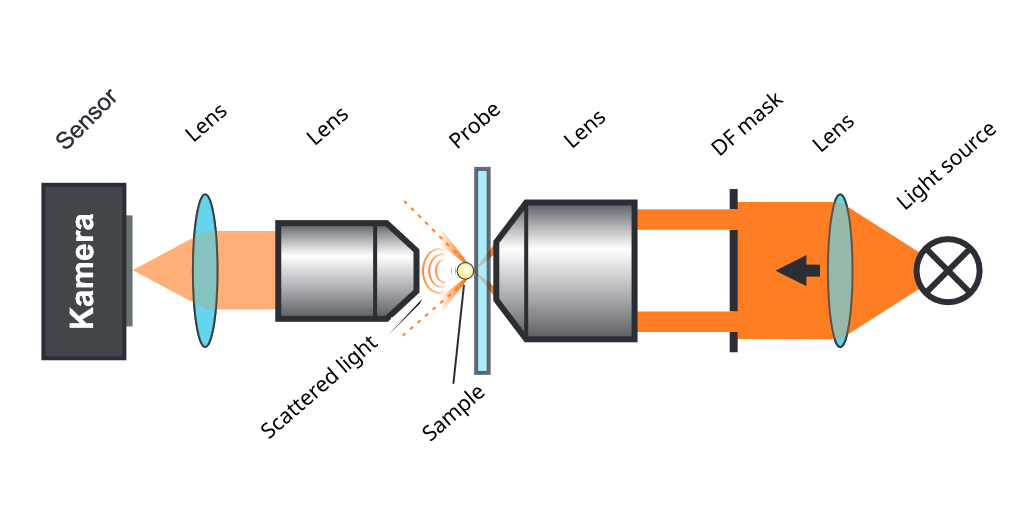
\includegraphics[width = \linewidth]{Bilder/Setup/MikroskopEdit.png}
    \caption{Schematic representation of the used dark-field microscope. From \cite{LehrstuhlExperimentalphysikIII.2023}}
    \label{fig:DarkFMicro}
\end{figure}

The first lense parallelizes the light. After this a dark field mask (DF mask) blocks the light which would directly enter in teh second lense of the microscope. The light which is transmitted by the DF mask is guided onto the sample and 
is scattered by the structure. This scattered light is picked up by the lense after the sample and converted to an image using the rest of the lenses. This picture is captured by the camera.

\subsection{Adjusting the setup}

The setup adjustment consists of multiple steps. Firstly, the positioning of the first lens is adjusted. Next, the second lens is focused on the sample, followed by guiding the beam into the spectrometer using two mirrors.

To adjust the position of the first lens, we incorporate a beam splitter in the beam path before the lens. The lens is then focused on the sample. To verify the focus we aim for a sharp image of the reflection, which can be observed through the beam splitter, as shown in Figure \ref{fig:subfig1}.
For this the position of the sample has to be changed using the millimeter screws until we see a the nano particles.


\begin{figure}[ht]
    \centering
    \begin{subfigure}{0.3\linewidth}
      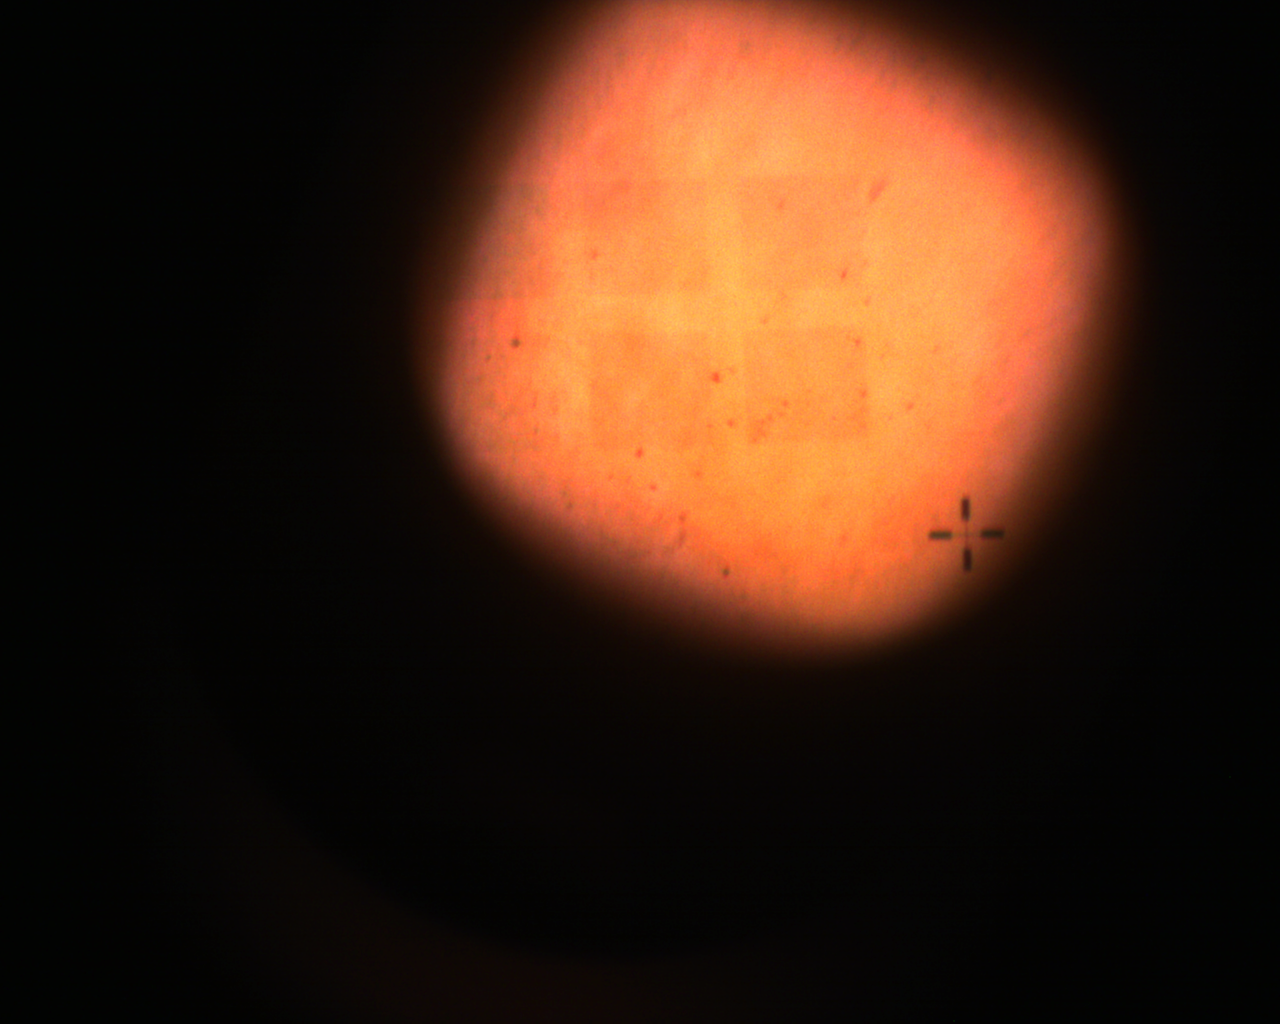
\includegraphics[width=\linewidth]{data/Gruppe2/image_0.png}
      \caption{}
      \label{fig:subfig1}
    \end{subfigure}
    \begin{subfigure}{0.3\linewidth}
      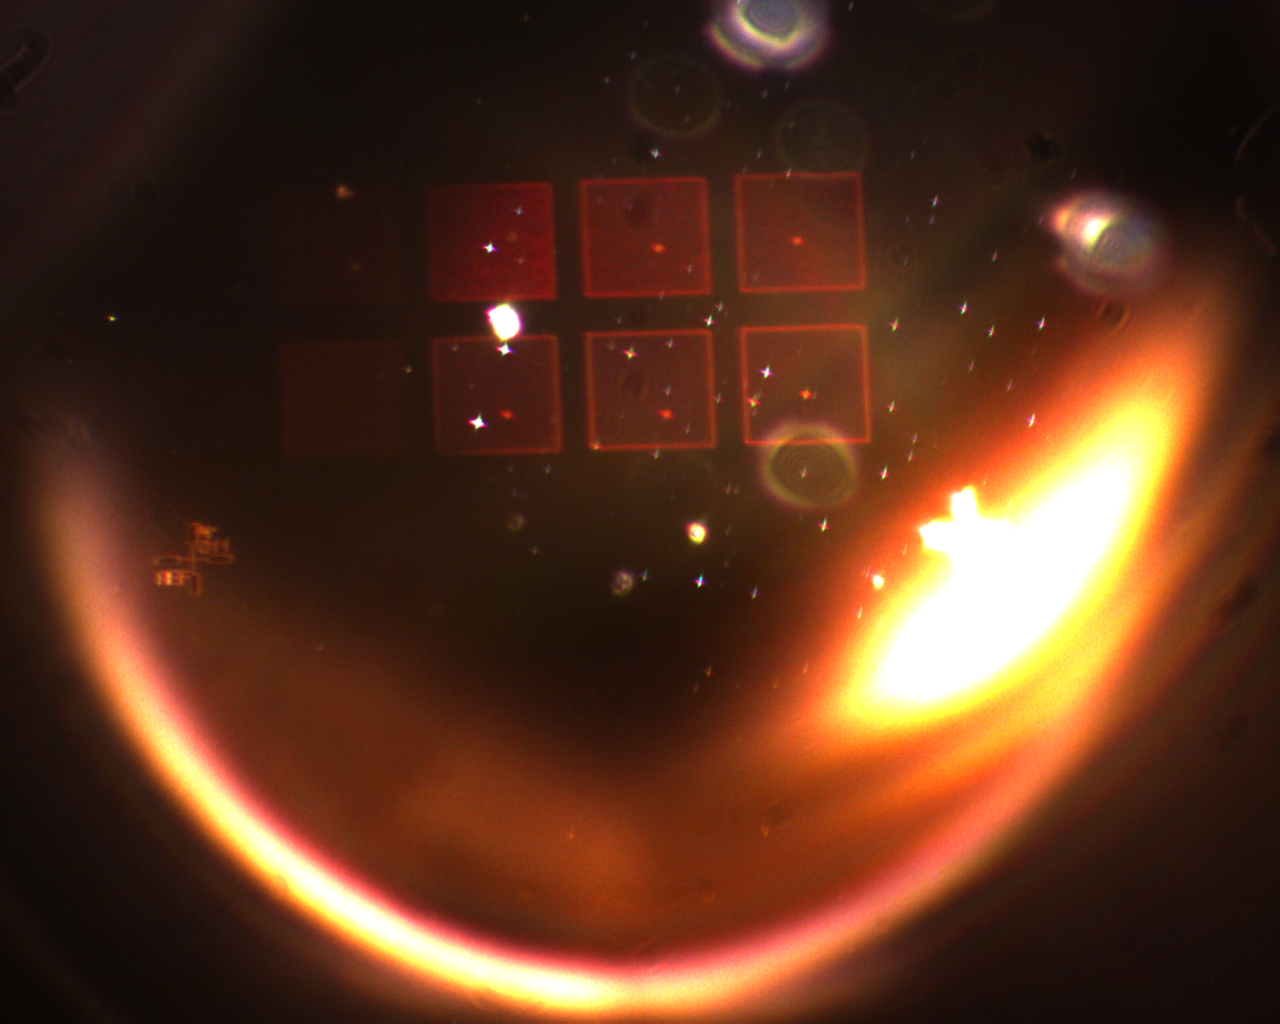
\includegraphics[width=\linewidth]{data/Gruppe2/image_1.png}
      \caption{}
      \label{fig:subfig2}
    \end{subfigure}
    \begin{subfigure}{0.3\linewidth}
      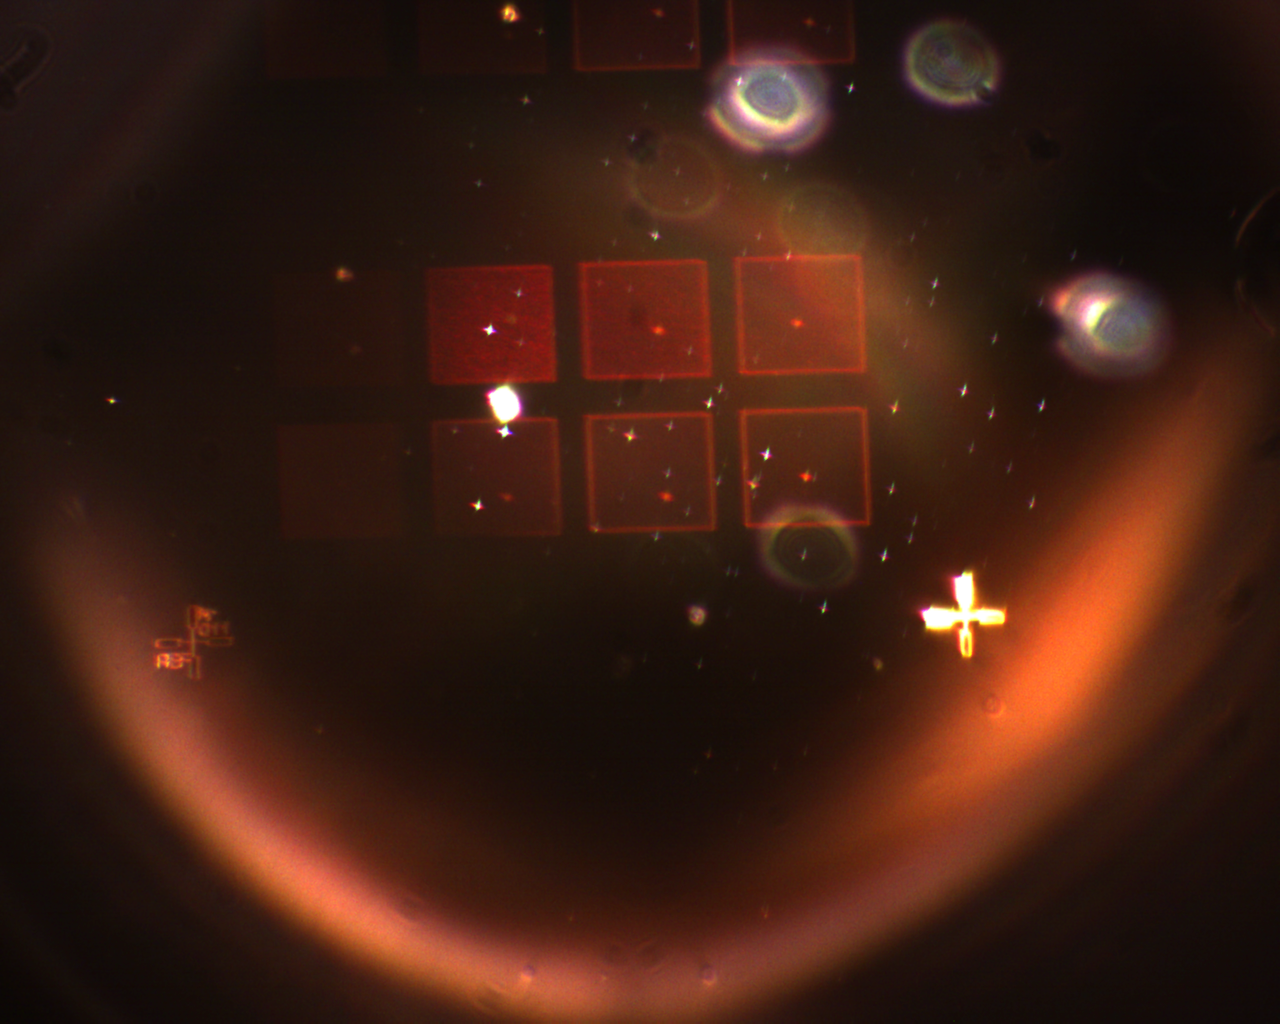
\includegraphics[width=\linewidth]{data/Gruppe2/image_2.png}
      \caption{}
      \label{fig:subfig3}
    \end{subfigure}

    \begin{subfigure}{0.3\linewidth}
      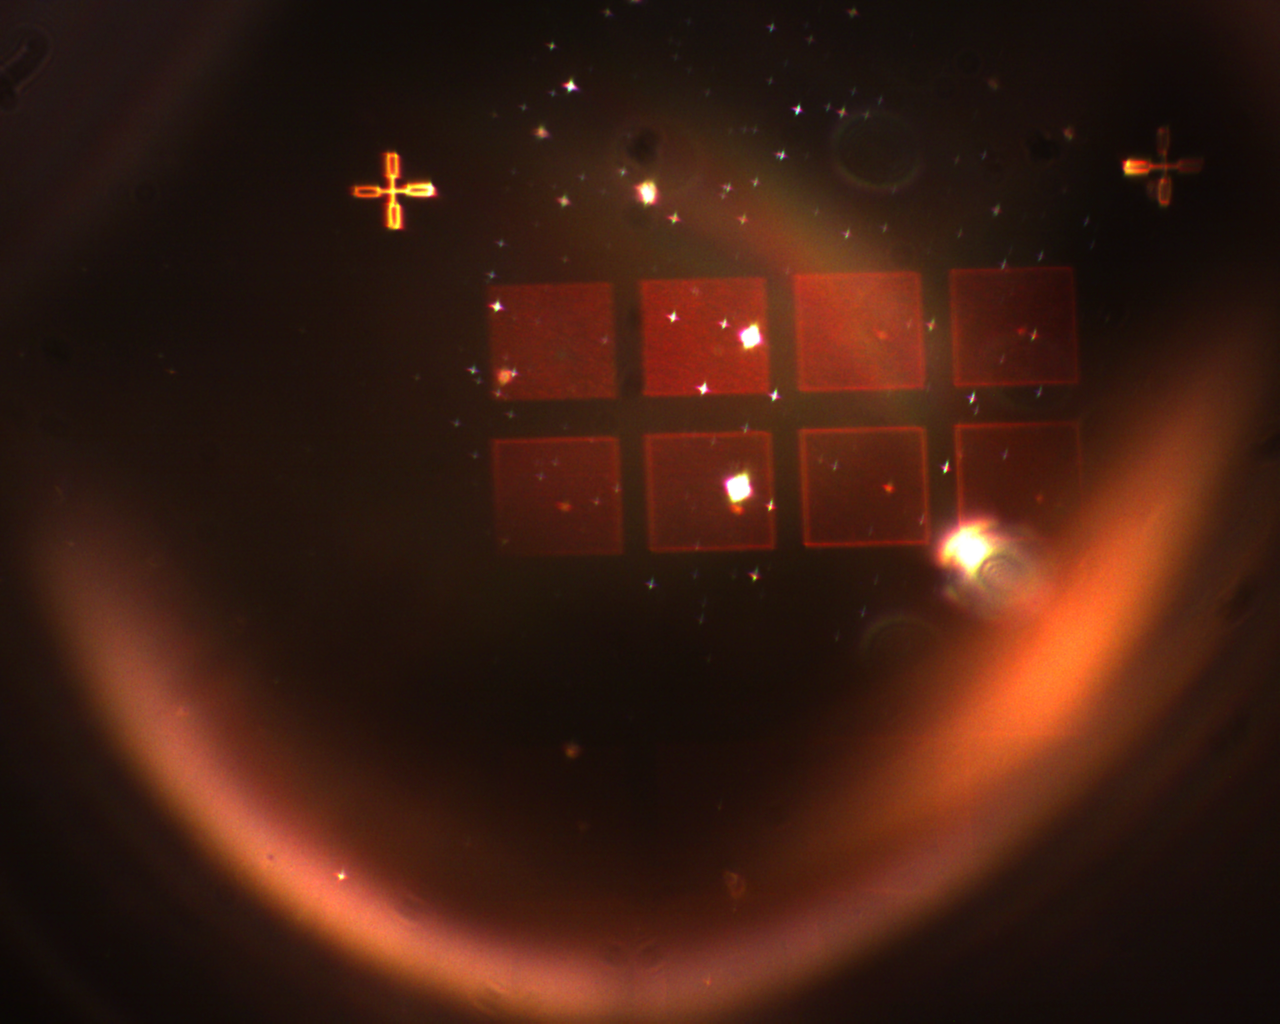
\includegraphics[width=\linewidth]{data/Gruppe2/image_3.png}
      \caption{}
      \label{fig:subfig4}
    \end{subfigure}
    \begin{subfigure}{0.3\linewidth}
      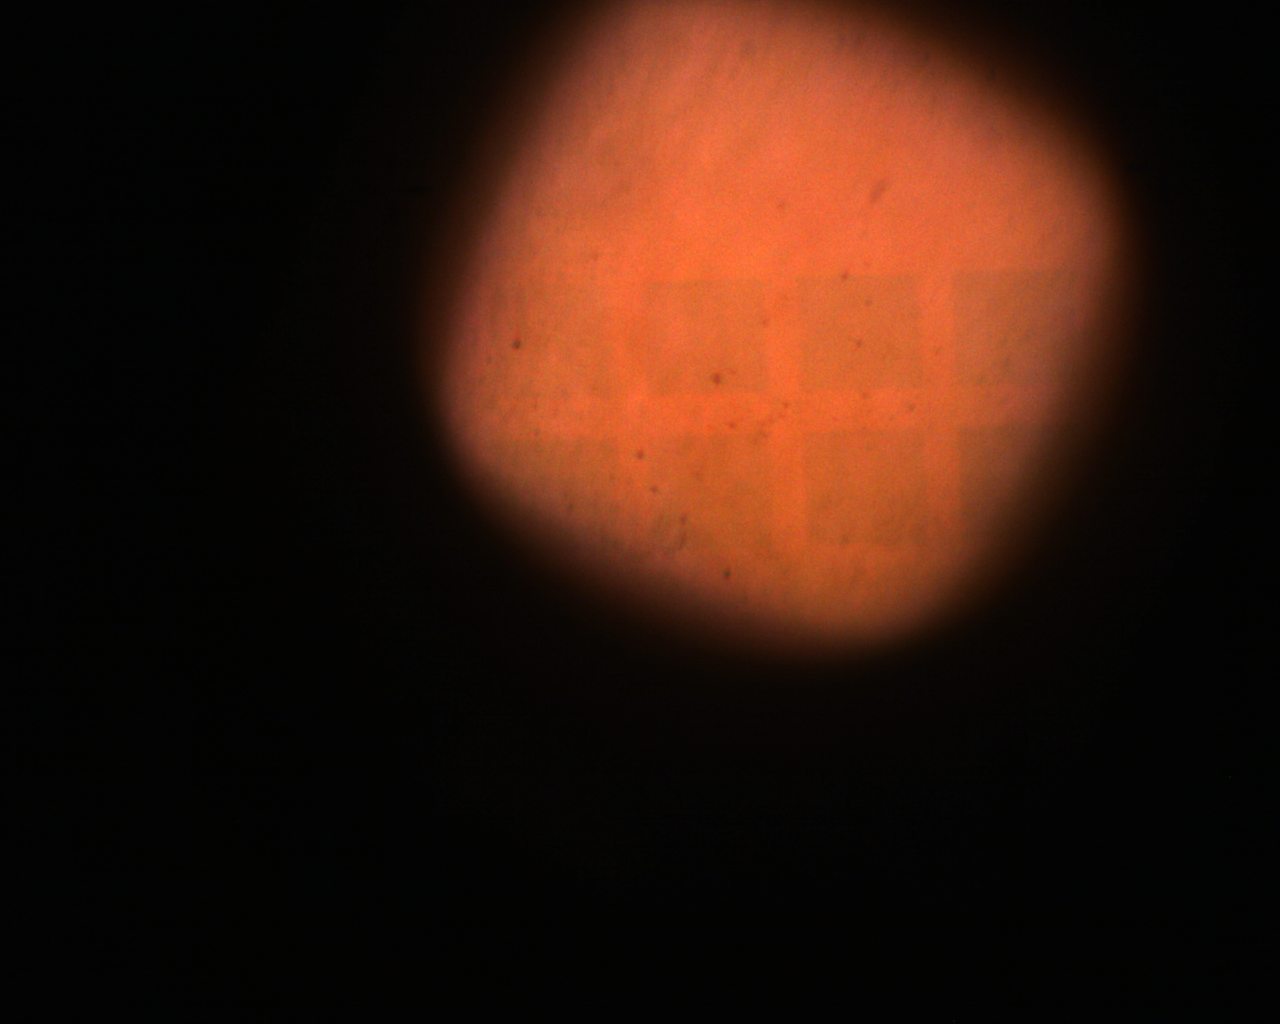
\includegraphics[width=\linewidth]{data/Gruppe2/image_4.png}
      \caption{}
      \label{fig:subfig5}
    \end{subfigure}
    \begin{subfigure}{0.3\linewidth}
      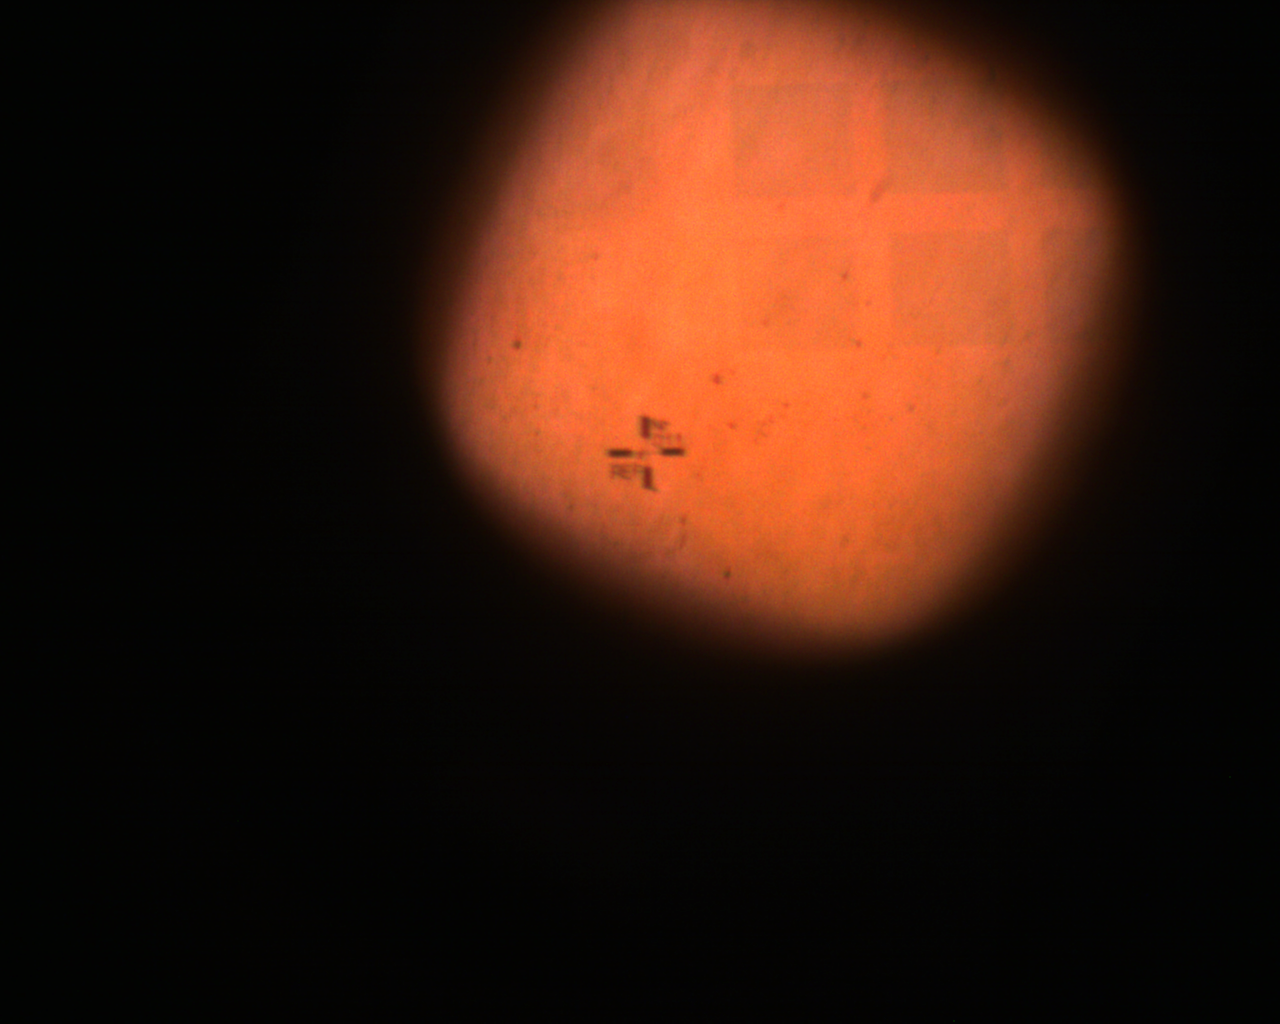
\includegraphics[width=\linewidth]{data/Gruppe2/image_5.png}
      \caption{}
      \label{fig:subfig6}
    \end{subfigure}


    \begin{subfigure}{0.3\linewidth}
      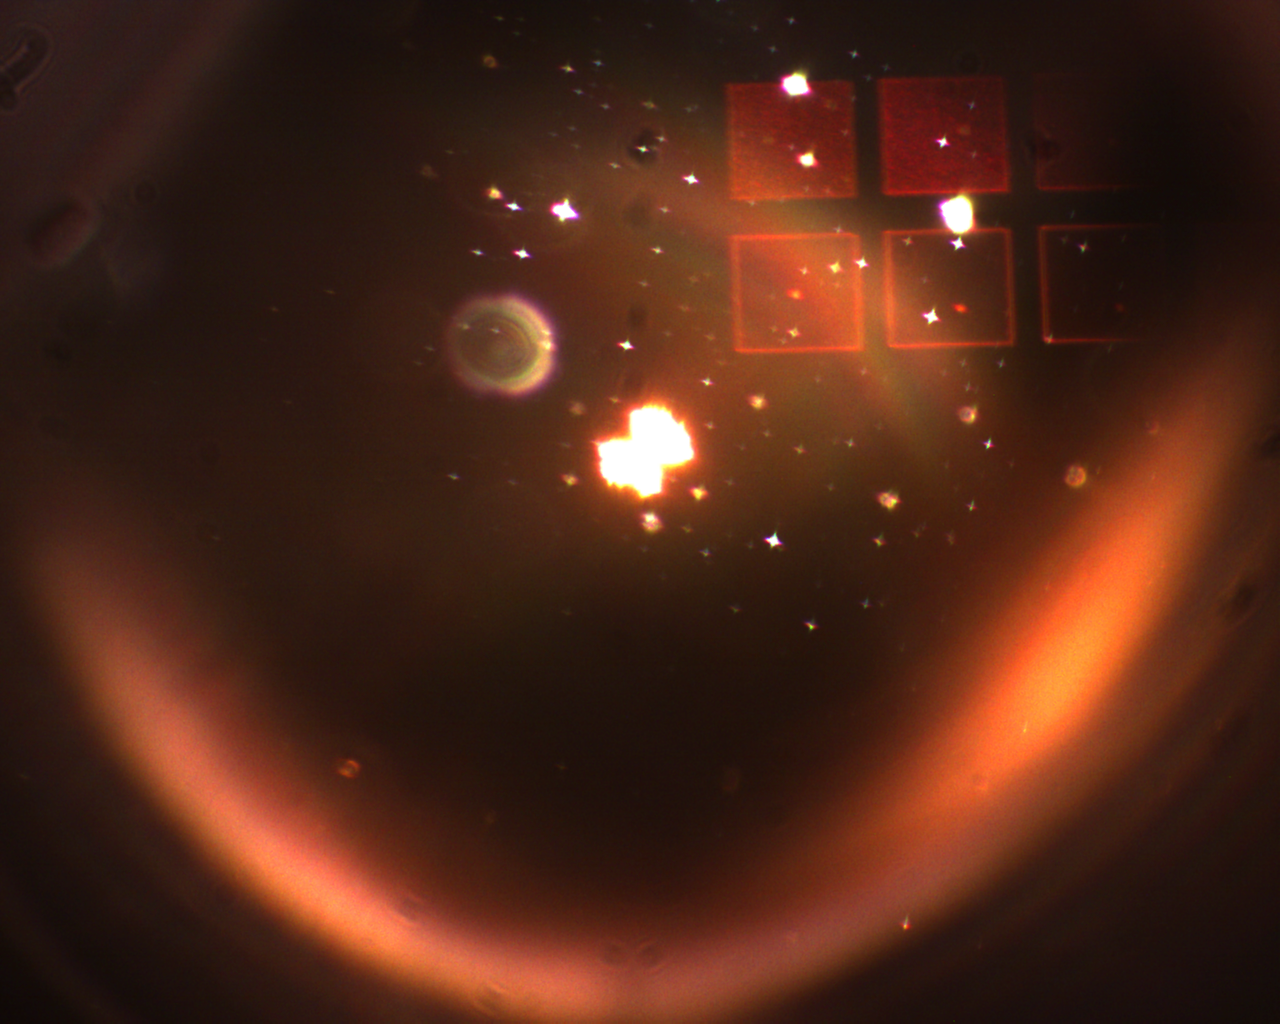
\includegraphics[width=\linewidth]{data/Gruppe2/image_6.png}
      \caption{Horizontal polarizations}
      \label{fig:subfig7}
    \end{subfigure}
    \begin{subfigure}{0.3\linewidth}
      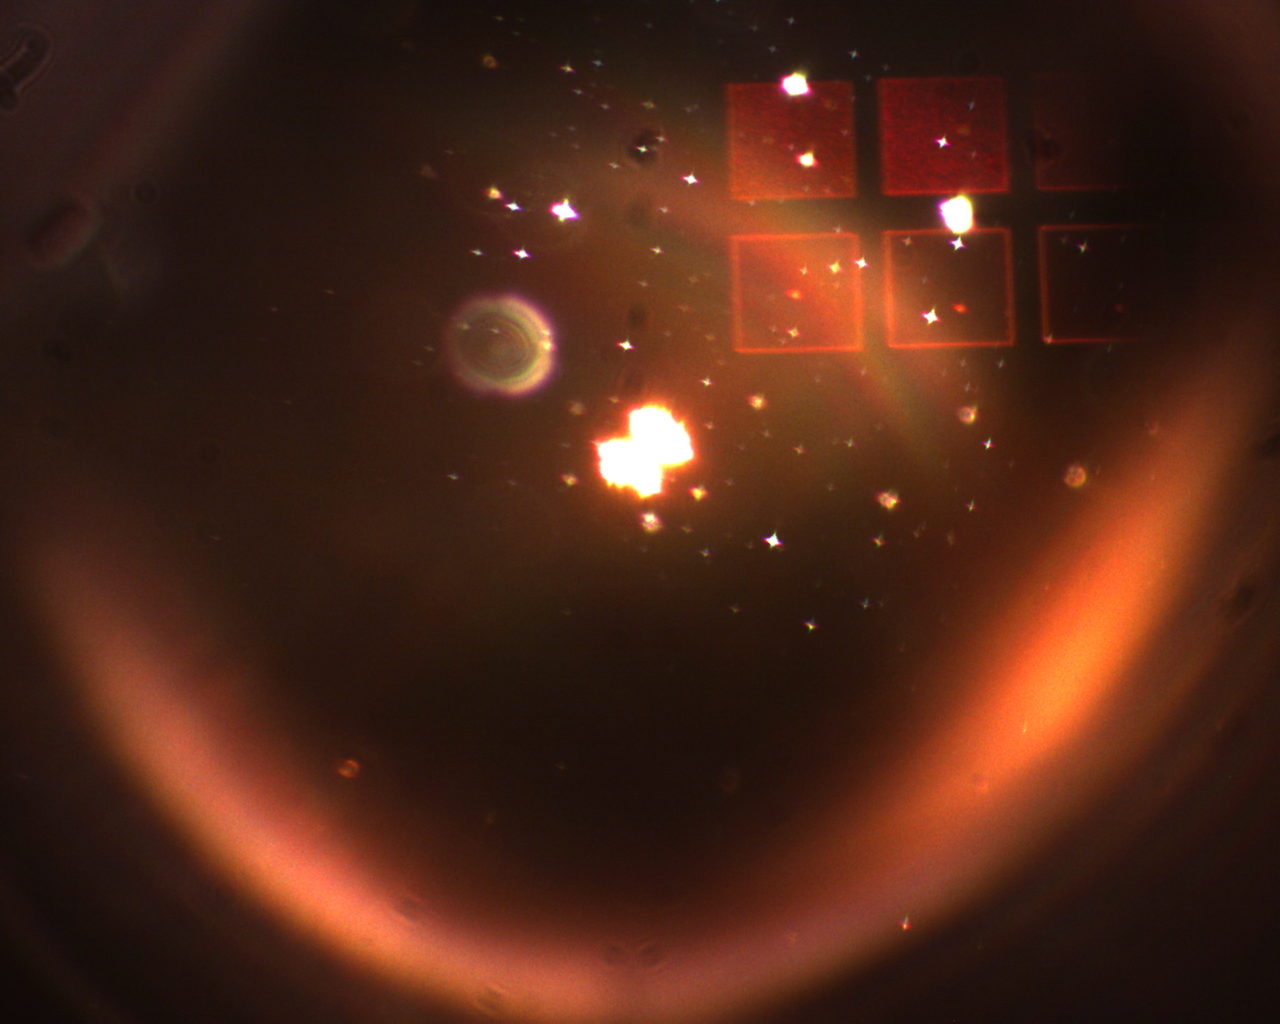
\includegraphics[width=\linewidth]{data/Gruppe2/image_7.png}
      \caption{Vertical polarizations}
      \label{fig:subfig8}
    \end{subfigure}
    \begin{subfigure}{0.3\linewidth}
      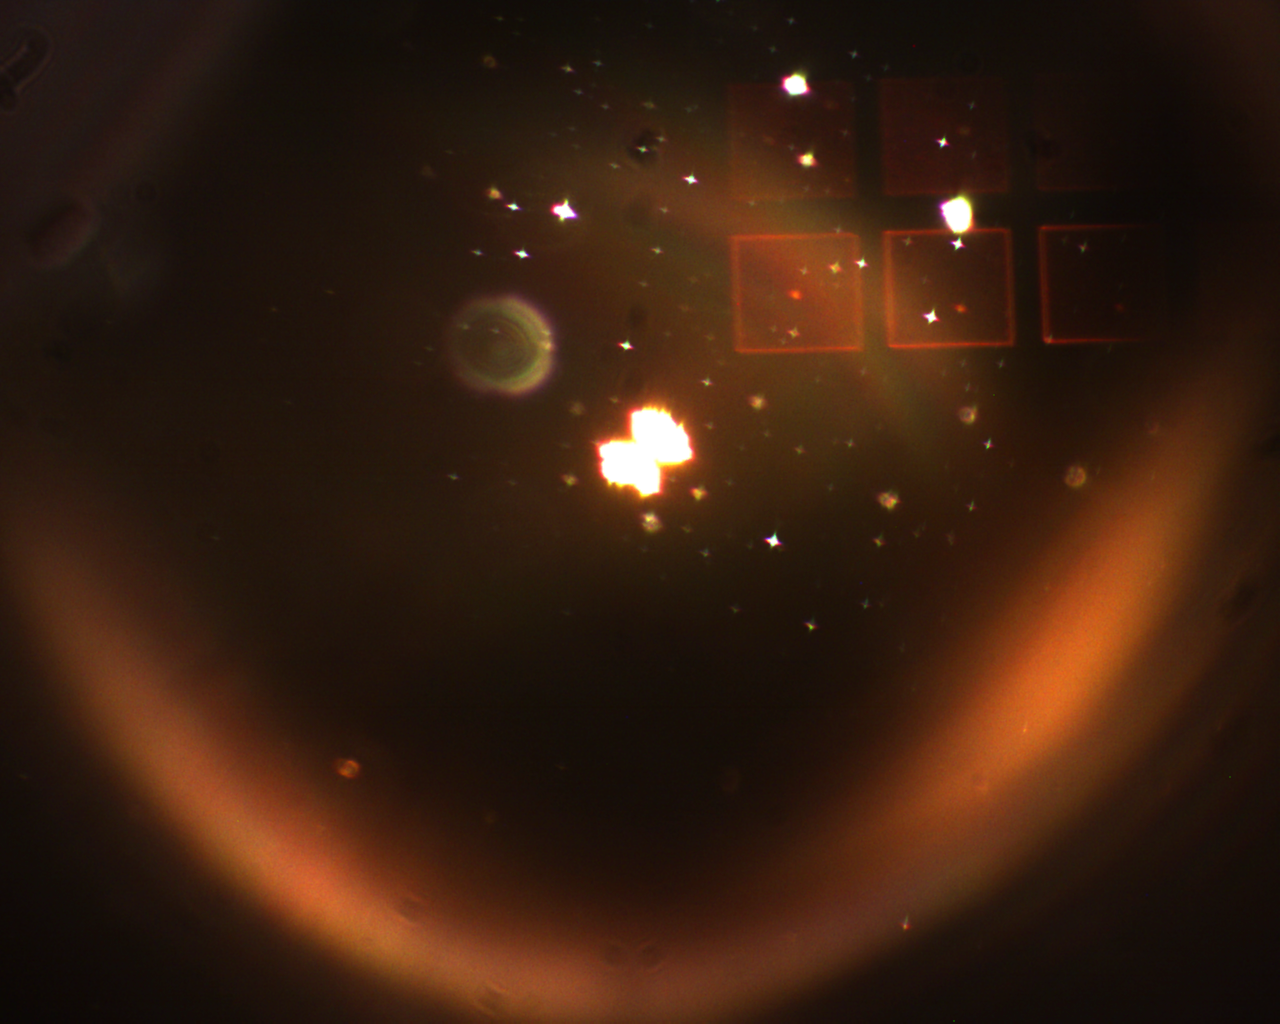
\includegraphics[width=\linewidth]{data/Gruppe2/image_8.png}
      \caption{}
      \label{fig:subfig9}
    \end{subfigure}
    
    \caption{The pictures were generated during adjustment of the setup. (a) shows the reflection of the film captured with a camera positioned at the place of the beam splitter. The pictures (b)-(i) ones were taken in transmission, after the adjustment of the second lens.}
    \label{fig:subfigure-grid}
\end{figure}

As a second step, the position of the second lens is optimized using a LASER. The LASER is quickly mounted instead of the LED. The diameter of the LASER spot is minimized by changing the distance of the second lens.

After inserting a second beam splitter following the second lens, we are able to view the transmission picture using a camera, as shown in \cref{fig:subfig2,fig:subfig3,fig:subfig4,fig:subfig5,fig:subfig6,fig:subfig7,fig:subfig8,fig:subfig9}. The contrast increasing effects
of the dark-field microscopy can be easily seen in \cref{fig:subfigure-grid} after placing the DF mask. The positioning of the mask gives artefact as can be seen in comparing \cref{fig:subfig2,fig:subfig9}. The sample is examined to determine its position by identifying the markers present non its edges. In \cref{fig:subfig7,fig:subfig8,fig:subfig9}, the marker with text can be seen in the bottom left corner. 
By comparing this to the plan for the sample depicted in \cref{fig:NanoDotSketch} and taking into account the orientation of the 
letters on the marker, we can tell that the sample is orientated as on the plan. When inserting polarizations filters as done in \cref{sub@fig:subfig7,sub@fig:subfig9}, we can not notice a difference in the scattering without numerical analysis. A slight shift in color might be visible.  
 

\begin{figure}[ht]
    \centering
    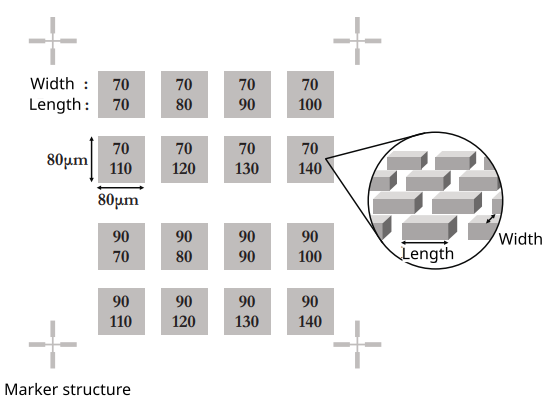
\includegraphics[width = 0.8\linewidth]{Bilder/Setup/SchemeDots.png}
    \caption{Schematic representation of the nano dot structure used. From \cite{LehrstuhlExperimentalphysikIII.2023}}
    \label{fig:NanoDotSketch}
\end{figure}

Afterwards, the beam is directed into the spectrometer by utilizing two mirrors. The slit is fully opened. Using the spectrometer, we examine a small image captured through the slit, which allows us to determine our location on the sample by identifying distinctive contaminants present. Once the sample position is determined, we reduce noise by closing the slit and manually positioning the sample using the second beam splitter and the camera to orient ourselves on the sample. When it comes to measurement, we remove both beam splitters.